% v4b (gfx2-stylist, 16 Nov 2026) = method_overview_v4a.tex (d587f4591155), one string swap from critic note DGX3_FIGS_CHECK_v1,
% agreed by story-lead in STRINGMAP_dgx3figs_v1_AGREED_storylead.md (f331fd96ef78): box title "Members who act" -> "Acting members".
% Nothing else changes. Build: python -I build_method_v4b.py <TEXT_LOAD_MAP_v1.md> <STRINGMAP_dgx3figs_v1_AGREED_storylead.md> <outdir>
% v4a (gfx2-stylist, 16 Nov 2026) = method_overview_source.tex (9c948fa952ee) with TEXT_LOAD_MAP_v1 (7c4a00644418) rows 1.1-1.7
% swapped in; nothing else changes. Build: python -I build_method_v4a.py <TEXT_LOAD_MAP_v1.md> <outdir>
% Method overview for the ATEKi MGEA paper (vector, deterministic).
% Knowledge sources are the members of a campaign; every subset of them is run as a campaign of its own,
% the measured table v(S) is divided by contribution measures, and organizational structure restricts
% which members combine. The measures are then read in organization-science terms.
% Compile on the DGX: ~/.local/bin/tectonic method_overview_source.tex  ->  method_overview_source.pdf, then copy it to method_overview_fig.pdf
\documentclass[tikz,border=4pt]{standalone}
\usetikzlibrary{arrows.meta,positioning,fit,calc,shapes.geometric,backgrounds}
\definecolor{mpblue}{HTML}{2E5FA3}
\definecolor{jgreen}{HTML}{009E73}
\definecolor{spurple}{HTML}{7A4DD8}
\definecolor{amber}{HTML}{E69F00}
\definecolor{ink}{HTML}{333333}
\definecolor{paleblue}{HTML}{EEF2F8}
\definecolor{palegold}{HTML}{F9F3E4}
\definecolor{palegrey}{HTML}{F4F4F4}
\begin{document}
\hyphenpenalty=10000 \exhyphenpenalty=10000
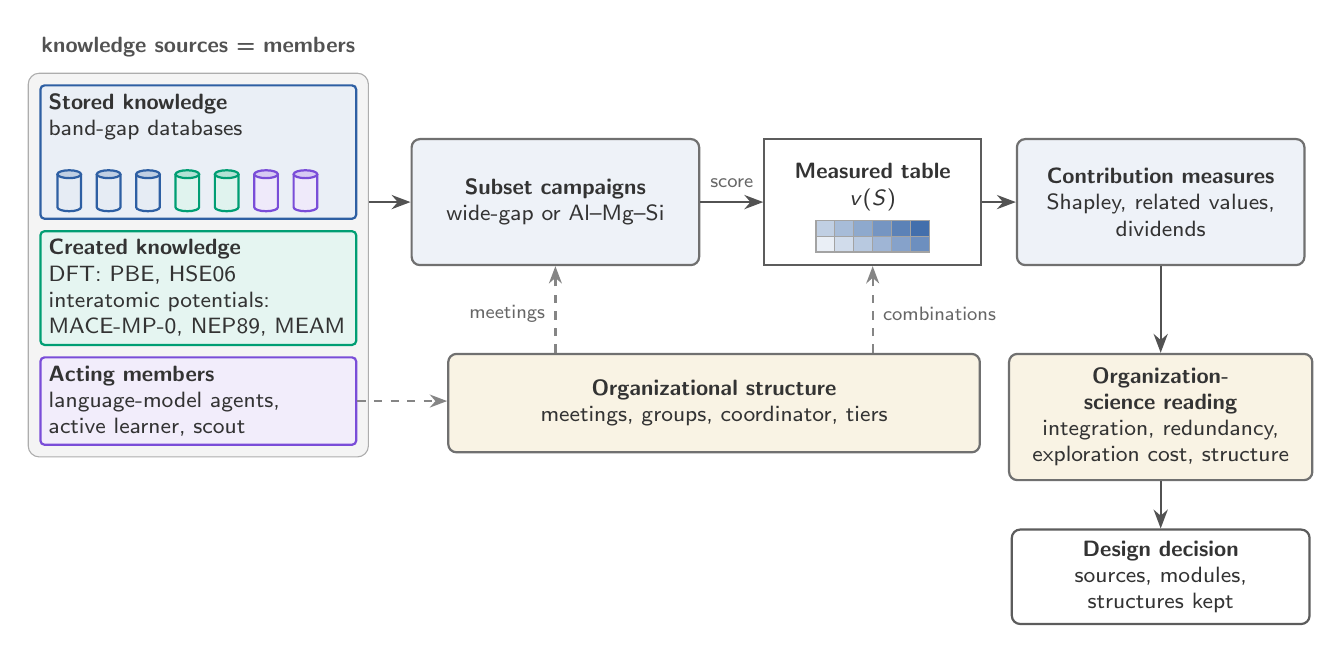
\begin{tikzpicture}[
  font=\sffamily\small,
  every node/.style={text=ink},
  member/.style={draw=#1, fill=#1!10, thick, rounded corners=1.5pt, text width=3.80cm, align=left,
                 inner sep=3pt, font=\sffamily\footnotesize, minimum height=0.95cm},
  db/.style={cylinder, shape border rotate=90, aspect=0.22, draw=#1, fill=#1!10, thick,
             minimum width=3.6mm, minimum height=5.2mm, inner sep=0pt},
  stage/.style={draw=ink!70, fill=#1, thick, rounded corners=3pt, align=center, inner sep=5pt,
                text width=3.3cm, minimum height=1.6cm, font=\sffamily\footnotesize},
  flow/.style={-{Stealth[length=2.4mm]}, thick, ink!85},
  logic/.style={-{Stealth[length=2.2mm]}, thick, ink!60, dashed},
  lab/.style={font=\sffamily\bfseries\footnotesize, text=ink!85},
  note/.style={font=\sffamily\fontsize{7.5}{9}\selectfont, text=ink!75, align=center}
]
% ---------------- members: knowledge sources --------------------------------------------------
\node[member=mpblue] (stored) {\textbf{Stored knowledge}\\band-gap databases\\[6.2mm]\mbox{}};
\foreach \c [count=\i] in {mpblue,mpblue,mpblue,jgreen,jgreen,spurple,spurple} {
  \begin{scope}[shift={($(stored.south west)+(-0.12+0.5*\i,0.16)$)}]
    \filldraw[draw=\c, fill=\c!12, thick] (-0.15,0.42) -- (-0.15,0) arc[start angle=180, end angle=360, x radius=0.15, y radius=0.05] -- (0.15,0.42);
    \filldraw[draw=\c, fill=\c!30, thick] (0,0.42) ellipse[x radius=0.15, y radius=0.05];
  \end{scope}
}
\node[member=jgreen, below=1.3mm of stored] (created) {\textbf{Created knowledge}\\DFT: PBE, HSE06\\interatomic potentials:\\MACE-MP-0, NEP89, MEAM};
\node[member=spurple, below=1.3mm of created] (agents) {\textbf{Acting members}\\language-model agents,\\active learner, scout};
\begin{scope}[on background layer]
  \node[draw=ink!40, fill=palegrey, rounded corners=4pt, inner sep=4pt, fit=(stored)(agents)] (members) {};
\end{scope}
\node[lab, above=0.8mm of members.north] {knowledge sources = members};

% ---------------- the measurement pipeline -----------------------------------------------------
\node[stage=paleblue, right=5.28mm of members.east, anchor=west, yshift=8mm] (run)
  {\textbf{Subset campaigns}\\wide-gap or Al--Mg--Si};
% measured table: sharp rectangle with a small grid
\node[draw=ink!80, fill=white, thick, right=8mm of run, text width=2.40cm, align=center, inner sep=5pt,
      minimum height=1.6cm, font=\sffamily\footnotesize] (table)
  {\textbf{Measured table}\\\textsl{v}(\textsl{S})\\[1.2mm]\phantom{x}};
\foreach \r in {0,1} \foreach \k in {0,...,5} {
  \draw[ink!45, fill=mpblue!\the\numexpr 10+12*\k+20*\r\relax] ($(table.south)+(-0.72+0.24*\k,0.18+0.2*\r)$) rectangle ++(0.24,0.2);
}
\node[stage=paleblue, right=4.28mm of table] (measures)
  {\textbf{Contribution measures}\\Shapley, related values,\\dividends};

\draw[flow] (members.east |- run.west) -- (run.west);
\draw[flow] (run) -- (table);
\draw[flow] (table) -- (measures);
\node[note, inner xsep=0pt, above=0.6mm of $(run.east)!0.5!(table.west)$] (score) {score};

% ---------------- organizational structure (restricts cooperation) ----------------------------
\node[stage=palegold, below=11mm of $(run.south)!0.5!(table.south)$, text width=6.4cm, minimum height=1.25cm] (struct)
  {\textbf{Organizational structure}\\meetings, groups, coordinator, tiers};
\draw[logic] (struct.north -| table.south) -- node[note, right, pos=0.45] (wc) {combinations} (table.south);
\draw[logic] (struct.north -| run.south) -- node[note, left, pos=0.45] (wm) {meetings} (run.south);
\draw[logic] (agents.east) -- (struct.west |- agents.east);

% ---------------- organization-science reading -------------------------------------------------
\node[stage=palegold, below=11mm of measures, text width=3.50cm, minimum height=1.25cm] (reading)
  {\textbf{Organization-science reading}\\integration, redundancy,\\exploration cost, structure};
\draw[flow] (measures) -- (reading);
\node[draw=ink!80, thick, fill=white, rounded corners=3pt, below=6mm of reading, text width=3.50cm, align=center,
      inner sep=4pt, font=\sffamily\footnotesize] (decide)
  {\textbf{Design decision}\\sources, modules,\\structures kept};
\draw[flow] (reading) -- (decide);
% ---- gate read-out (log only; draws nothing)
\newdimen\gA \newdimen\gB
\def\gx#1#2#3#4#5{\pgfextractx{\gA}{\pgfpointanchor{#2}{#3}}\pgfextractx{\gB}{\pgfpointanchor{#4}{#5}}%
  \advance\gB by -\gA \typeout{GATE #1 \the\gB}}
\gx{members_run}{members}{east}{run}{west}
\gx{run_score}{run}{east}{score}{west}
\gx{score_table}{score}{east}{table}{west}
\gx{struct_reading}{struct}{east}{reading}{west}
\gx{wc_arrow}{wc}{east}{measures}{south}
\gx{members_wm}{members}{east}{wm}{west}
\gx{agents_struct}{agents}{east}{struct}{west}
\end{tikzpicture}
\end{document}
